\chapter{Analisis Masalah Dan Rancangan Solusi}

\par Dalam mengadakan kompetisi \textit{competitive programming} diperlukan sebuah sistem \textit{online judge}. Sistem \textit{online judge} memerlukan dua buah komponen utama yaitu \textit{autograder} dan sistem manajemen kompetisi. Sistem manajemen kompetisi memberikan layanan yang berhubungan dengan kompetisi seperti melihat soal, mengirim jawaban, membuat klarifikasi, dan melihat \textit{scoreboard}. Sistem \textit{autograder} berfungsi untuk melakukan penilaian terhadap jawaban yang telah dikirim secara \textit{realtime}.

\section{Sistem \textit{Autograder}}

\par Sistem manajemen kompetisi memerlukan \textit{autograder} untuk menilai jawaban peserta kompetisi secara otomatis. Sistem \textit{online judge} yang sering digunakan saat ini menggunakan \textit{autograder} yang dipasang oleh juri pada beberapa komputer yang sudah disediakan oleh juri. Pada Tugas Akhir ini akan diciptakan sistem \textit{autograder} yang dapat berjalan pada komputer peserta. Komputer peserta akan bertindak sebagai \textit{worker} yang menjalankan sistem \textit{autograder}. \textit{Worker} adalah komputer yang digunakan oleh sistem \textit{autograder} untuk melakukan penilaian terhadap jawaban peserta. Dalam Tugas Akhir ini, komputer peserta adalah \textit{worker} dari sistem \textit{autograder}. Terdapat beberapa aspek yang perlu diperhatikan dalam mengembangkan sistem \textit{autograder} seperti pengukuran waktu dan memori, \textit{load balancing}, evaluasi jawaban peserta, dan pengiriman \textit{test-case} ke \textit{worker}

\subsection{Pengukuran Waktu Dan Memori} \label{subsec:time-memory-measure}

\par Komputer peserta memiliki spesifikasi yang berbeda-beda. Perbedaan spesifikasi tersebut menimbulkan beberapa perbedaan ketika sebuah program yang sama dieksekusi. Program yang sama dengan masukan yang sama dapat berjalan dengan waktu dan memori yang berbeda pada komputer yang berbeda. Komputer yang memiliki \textit{clock-speed} yang lebih tinggi akan menjalankan program lebih cepat. Komputer yang memiliki \textit{core} lebih banyak juga akan menjalankan program parallel dengan lebih cepat. Selain itu, ukuran \textit{cache} dari komputer juga memengaruhi kecepatan waktu eksekusi. Kebutuhan memori dari suatu program juga ditentukan oleh spesifikasi komputer. Komputer dengan arsitektur 64-bit umumnya memerlukan memori yang lebih besar dibandingkan arsitektur 32-bit. Oleh karena itu, program peserta yang dieksekusi pada komputer yang berbeda akan memerlukan waktu dan memori yang berbeda pula.

\par Diperlukan sistem pengukuran waktu yang adil sehingga program peserta yang benar akan dianggap benar di setiap komputer. Begitu juga program peserta yang salah akan dianggap salah di setiap komputer. Terdapat beberapa teknik yang dapat digunakan untuk mengukur waktu eksekusi jawaban peserta.

\subsubsection{Spesifikasi CPU dan Sistem Operasi}

\par Kecepatan eksekusi sebuah program ditentukan dari \textit{clock-speed}, dan \textit{cache} dari CPU. Jika program peserta hanya diberikan satu buah \textit{core} dari CPU, maka jumlah \textit{core} dari CPU tidak perlu diperhatikan lagi. Kecepatan eksekusi program peserta dapat diukur dari spesifikasi CPU peserta. Komputer dengan \textit{clock-speed} dan ukuran \textit{cache} yang rendah akan diberikan batasan waktu yang lebih lama. Arsitektur setiap komputer juga berbeda-beda. Komputer dengan arsitektur 64-bit umumnya memerlukan memori yang lebih besar. Dengan mengetahui arsitektur komputer, kebutuhan memori dapat diperkirakan.

\par Pada penilaian jawaban peserta, diperlukan pengukuran waktu dan memori yang sangat akurat. Pengukuran waktu atau memori yang tidak akurat akan menimbulkan ketidakadilan kepada peserta. Dengan hanya memerhatikan spesifikasi dari CPU dan sistem operasi pada komputer, pengukuran waktu dan memori yang akurat sulit dilakukan. Program yang berjalan pada sistem operasi 64-bit tidak selalu memerlukan memori dua kali dari program yang berjalan pada sistem operasi 32-bit. Kebutuhan memori bergantung pada isi dari program yang dijalankan. Selain itu, menentukan batasan waktu program dari \textit{clock-speed} dan \textit{cache} tidak mudah dilakukan. 

\subsubsection{CPU \textit{Benchmarking}}

\par \textit{Benchmarking} dapat dilakukan untuk mengukur kinerja CPU dengan menggunakan sebuah program \textit{test}. Program \textit{test} dapat dijalankan pada CPU untuk mengukur waktu eksekusinya. Program \textit{test} yang dijalankan pada komputer pengguna akan dicatat jumlah instruksi dan waktunya. Jumlah instruksi dan waktu yang dibutuhkan untuk menjalankan program \textit{test} dapat digunakan untuk mengukur kinerja CPU. Batas waktu dari jawaban peserta kemudian akan ditentukan berdasarkan hasil pengetesan tersebut.

\par \textit{Benchmarking} pada komputer peserta memiliki celah keamanan. Peserta bisa saja menjalankan program yang berat ketika proses \textit{benchmarking} dilakukan. Hal ini akan menyebabkan waktu eksekusi menjadi lambat dan dapat meningkatkan batasan waktu dari jawaban peserta. Hal ini dapat dihindari dengan cara melarang peserta menilai jawabannya sendiri dan hanya boleh menilai jawaban peserta lain sehingga peserta tidak memiliki alasan untuk melakukan kecurangan pada saat \textit{benchmarking}. Akan tetapi hal ini masih menimbulkan celah keamanan. Peserta dapat mematikan jaringan komputernya sehingga tidak dapat bertindak sebagai \textit{worker}. Hal ini menyebabkan berkurangnya \textit{worker} yang dapat digunakan untuk melakukan penilaian.

\subsubsection{Membandingkan Dengan Solusi Juri} \label{subsec:time-memory-measure-compare-with-jury}

\par Teknik \textit{benchmarking} sebenarnya efektif untuk digunakan. Pada teknik \textit{benchmarking}, permasalahan utamanya adalah bagaimana menghindari kecurangan peserta. Untuk mencegah peserta mematikan jaringan komputernya, setiap peserta perlu menilai jawabannya sendiri. Peserta yang mematikan jaringan komputernya tidak akan dapat menilai jawabannya sehingga merugikan dirinya sendiri.

\par Permasalahan lain yang timbul adalah peserta dapat menjalankan program yang berat ketika \textit{benchmarking} dilakukan. Hal ini menyebabkan hasil \textit{benchmarking} menunjukkan waktu eksekusi yang lama sehingga batas waktu dari jawaban peserta akan dinaikkan. Untuk menghindari hal ini, benchmarking dapat dilakukan bersamaan dengan proses eksekusi jawaban peserta. \textit{Worker} akan menjalankan program solusi juri dan program solusi peserta dalam waktu bersamaan. Jika program peserta memiliki waktu eksekusi dan memori yang tidak jauh berbeda dengan juri maka solusi peserta dianggap sesuai batasan. Keluaran program peserta kemudian akan dibandingkan dengan keluaran program juri untuk menentukan kebenarannya.

\begin{figure}
    \centering
    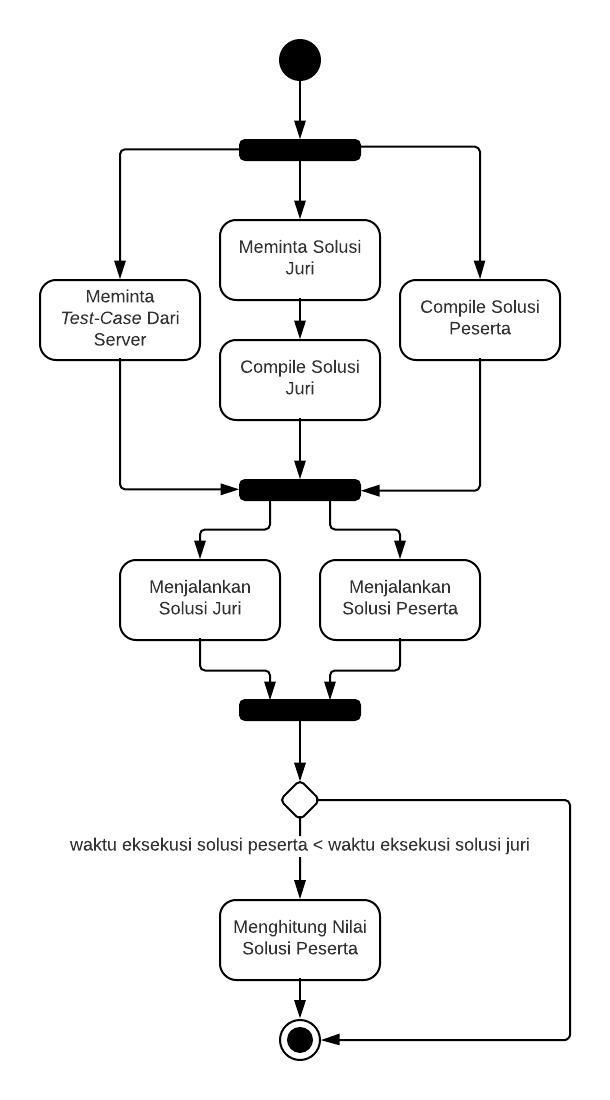
\includegraphics[width=0.5\textwidth]{images/cpu-time-counting}
    \caption{Diagram Aktivitas Penilaian Solusi Peserta}
    \label{fig:cpu-time-counting}
\end{figure}

\par Dengan membandingkan program solusi peserta dengan program solusi juri pada saat yang bersamaan, perhitungan waktu dan memori yang akurat dapat dilakukan. Meskipun peserta menjalankan program yang berat pada saat penilaian dilakukan, perbandingan waktu eksekusi dari program solusi juri dengan program solusi peserta akan tetap sama. Oleh karena itu, teknik ini akan digunakan untuk melakukan pengukuran waktu dan memori dalam menyelesaikan Tugas Akhir ini. Gambar \ref{fig:cpu-time-counting} menjelaskan proses penilaian jawaban peserta dengan membandingkan dengan program solusi juri. 

\subsection{\textit{Load Balancing}}

\par Dalam membangun sistem \textit{autograder}, diperlukan pembagian kerja kepada \textit{worker-worker} yang ada. \textit{Worker} yang dimaksud adalah komputer yang bekerja melakukan penilaian jawaban peserta. Dalam Tugas Akhir ini, \textit{worker} merupakan komputer peserta. Karena spesifikasi komputer tiap \textit{worker} berbeda-beda, diperlukan teknik pembagian kerja yang adil kepada seluruh peserta dan seluruh \textit{worker}. Selain itu aspek keamanan juga perlu diperhatikan karena jawaban peserta akan dikirimkan ke \textit{worker} lain. Terdapat beberapa pendekatan pembagian kerja yang dapat digunakan, yaitu: \textit{push-based}, \textit{pull-based}, dan \textit{self-grading}.

\begin{figure}
    \centering
    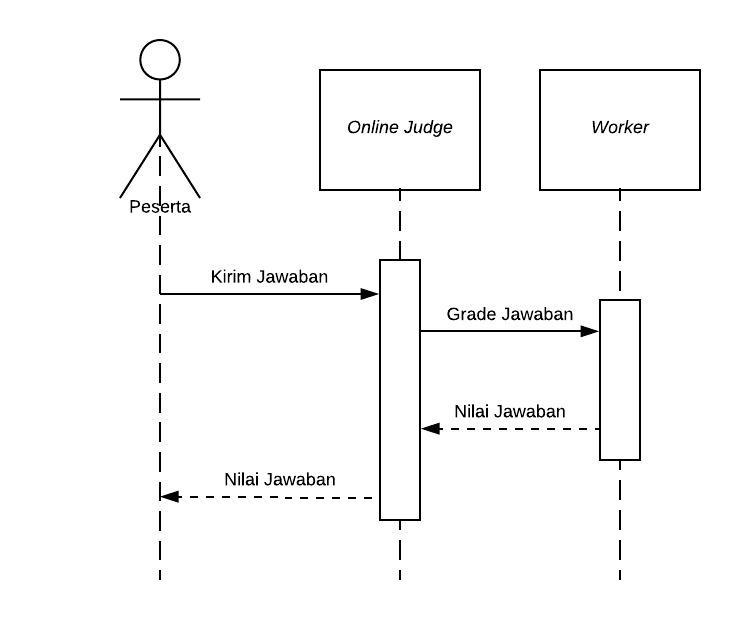
\includegraphics[width=0.75\textwidth]{images/load-balancing-push}
    \caption{\textit{Push-Based Load Balancer}}
    \label{fig:load-balancing-push}
\end{figure}

\par Pada pendekatan \textit{push-based}, sistem \textit{autograder} memerlukan sebuah \textit{master} yang akan membagikan pekerjaan ke seluruh \textit{worker}. \textit{Master} akan menentukan \textit{worker} mana yang akan diberikan suatu pekerjaan. Dengan menggunakan metode ini, \textit{master} perlu mengetahui informasi \textit{resource} dari seluruh \textit{worker} yang ada. Setiap \textit{worker} perlu mengirimkan informasi \textit{resource}-nya kepada \textit{master}. Metode ini cukup sulit untuk dilakukan karena perlunya mengimplementasikan algoritma \textit{load balancing} pada \textit{master}. Gambar \ref{fig:load-balancing-push} menggambarkan alur pembagian kerja dengan metode \textit{push-based}.

\begin{figure}
    \centering
    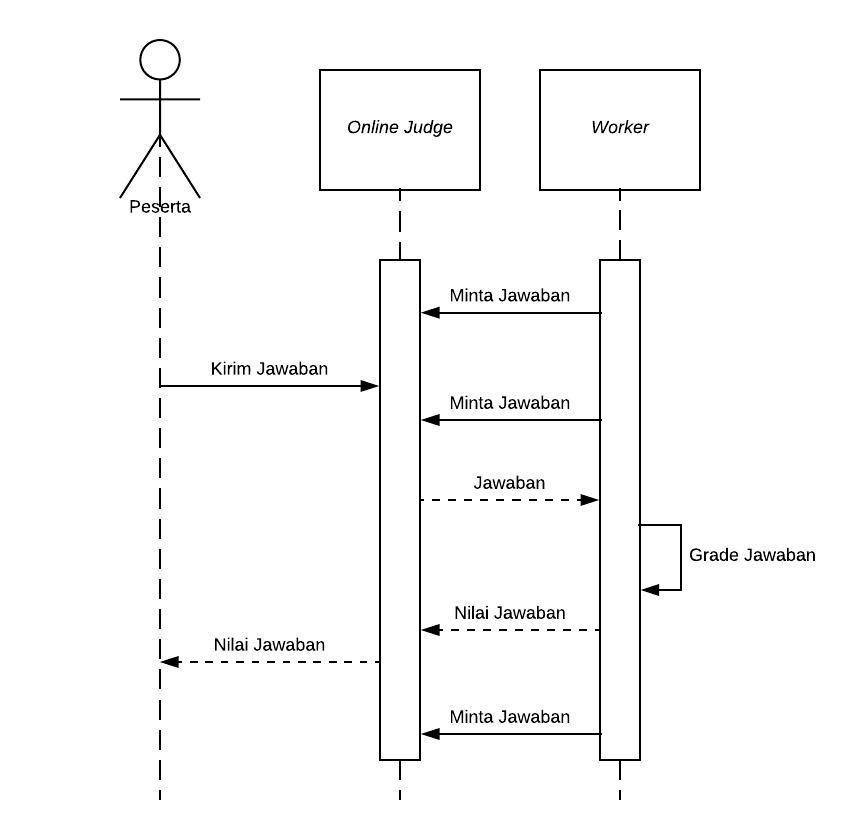
\includegraphics[width=0.75\textwidth]{images/load-balancing-pull}
    \caption{\textit{Pull-Based Load Balancer}}
    \label{fig:load-balancing-pull}
\end{figure}

\par Pada pendekatan \textit{pull-based}, diperlukan juga sebuah \textit{master} yang akan menyimpan seluruh pekerjaan yang perlu diselesaikan. Berbeda dengan pendekatan \textit{push-based} dimana \textit{master} lah yang memberikan \textit{worker} pekerjaan. Pada pendekatan \textit{pull-based}, \textit{worker} yang sedang tersedia akan meminta pekerjaan kepada \textit{master}. Dengan pendekatan ini, pembagian pekerjaan akan menjadi rata dengan sendirinya. Metode ini lebih mudah untuk diimplementasikan dibanding dengan metode \textit{push-bashed} karena tidak perlu membuat algoritma \textit{load balancing}. Gambar \ref{fig:load-balancing-pull} menggambarkan alur pembagian kerja dengan metode \textit{pull-based}.

\par Selain pendekatan \textit{push-based} dan \textit{pull-based}, terdapat pendekatan lain yang lebih sederhana yaitu \textit{self-grading}. Pada \textit{self-grading}, peserta akan menilai jawabannya sendiri. Dengan menggunakan pendekatan ini, tidak diperlukan adanya \textit{master}. Selain itu, metode \textit{self-grading} lebih adil dibandingkan dengan metode \textit{push-based} dan \textit{pull-based}. Pada dua metode lainnya, peserta dapat mengirimkan jawaban secara terus menerus kepada sistem \textit{autograder} sehingga membanjiri sistem dan menimbulkan berkurangnya kinerja sistem. Dengan metode \textit{self-grading}, peserta yang mengirimkan jawaban secara terus menerus tidak akan membanjiri sistem dan hanya memperlambat proses penilaian jawabannya sendiri. Pada bagian \ref{subsec:time-memory-measure} dan \ref{subsec:time-memory-measure-compare-with-jury} juga sudah dijelaskan bahwa pada Tugas Akhir ini setiap peserta akan menilai jawabannya sendiri. Oleh karena itu, pada Tugas Akhir ini akan digunakan teknik \textit{self-grading}. 

\subsection{Evaluasi Jawaban Menggunakan Sandbox}

\par Dalam melakukan penilaian terhadap jawaban peserta, diperlukan adanya proses kompilasi dan eksekusi terhadap program yang dikirimkan peserta. Proses kompilasi dan eksekusi ini akan dijalankan pada \textit{worker}. Proses ini dapat membahayakan lingkungan \textit{worker} jika peserta mengirimkan kode program yang berbahaya. Untuk menghindari kerusakan pada \textit{worker}, proses ini perlu diisolasi sehingga tidak berpengaruh pada lingkungan \textit{worker}. Teknik untuk mengisolasi proses eksekusi program ini dinamakan \textit{sandboxing}. Terdapat beberapa teknik \textit{sandboxing} yang dapat digunakan.

\subsubsection{Menggunakan \textit{Virtual Machine}}

\par \textit{Virtual machine} memberikan isolasi kepada program pada tingkat \textit{hardware}. Komputer yang ada pada saat ini memiliki \textit{hypervisor} yang dapat digunakan untuk mensimulasikan \textit{hardware} dari komputer. Dengan menggunakan \textit{virtual machine}, komputer dapat menjalankan sistem operasi virtual di atas sistem operasi yang sedang berjalan. \textit{Virtual machine} memberikan layanan isolasi yang sangat aman.

\par Meskipun keamanan \textit{virtual machine} sangat tinggi, akan tetapi banyak \textit{overhead} yang ditimbulkan. Untuk menyalakan \textit{virtual machine}, membutuhkan waktu yang lama dan memori yang cukup besar. Selain itu, diperlukan adanya sistem operasi baru yang berjalan di atas \textit{virtual machine} yang dibuat. Hal ini menyebabkan proses penilaian jawaban peserta menjadi lambat dan membutuhkan sangat banyak memori.

\subsubsection{Menggunakan \textit{Cgroup}, \textit{Chroot} dan \textit{Namespace}}

\par \textit{Cgroup}, \textit{chroot} dan \textit{namespace} merupakan suatu fitur pada linux yang memungkinkan penggunanya untuk mengeksekusi program secara terisolasi. \textit{Cgroup} dapat memberikan batasan \textit{resource} seperti IO, memory dan CPU kepada suatu program sehingga tidak membebani program lain. \textit{Chroot} memberikan isolasi \textit{filesystem} pada suatu program sehingga program yang berjalan di dalam \textit{chroot} tidak dapat mengakses \textit{filesystem} yang berada di luar \textit{chroot}. \textit{Namespace} memisahkan program pada linux menjadi beberapa partisi dan program pada sebuah partisi hanya dapat mengetahui program lain yang berada dalam partisi tersebut. Dengan menggabungkan ketiga fitur linux ini, dapat dibuat \textit{sandbox} yang cukup untuk mengeksekusi jawaban peserta.

\par Dengan menggunakan teknik ini, penilaian jawaban peserta dapat dilakukan secara aman dengan sedikit \textit{overhead}. Teknik ini sudah digunakan oleh teknologi \textit{container} untuk mengisolasi program. Oleh karena itu, isolasi program dengan \textit{cgroup}, \textit{chroot} dan \textit{namespace} dipilih dalam Tugas Akhir ini.

\subsection{Pengiriman \textit{Test-Case} Ke \textit{Worker}} \label{subsec:sending-test-case-to-worker}

\par Dalam melakukan penilaian jawaban peserta perlu adanya pengiriman \textit{test-case} dari \textit{server} ke \textit{worker}. \textit{Test-case} merupakan informasi yang digunakan untuk menentukan kebenaran jawaban peserta sehingga informasi ini bersifat rahasia dan tidak boleh diketahui oleh peserta maupun orang lain di luar kompetisi. \textit{Test-case} digunakan sebagai masukan pada saat menjalankan program solusi peserta dan juri. Kebenaran dari solusi peserta dinilai dari keluaran yang dihasilkan. Salah satu cara untuk menilai apakah program peserta tersebut benar atau tidak adalah dengan membandingkan dengan keluaran dari program solusi juri. Jika keluaran solusi peserta sama seperti keluaran solusi juri, maka solusi peserta akan dianggap benar. Akan tetapi, seringkali keluaran dari program solusi peserta tidak harus sama persis dengan solusi juri. Soal pada \textit{competitive programming} seringkali memiliki lebih dari satu solusi yang sah dan tidak mungkin untuk menuliskan semua solusi satu per satu. Oleh karena itu, diperlukan juga adanya program \textit{checker} yang digunakan untuk menentukan kebenaran solusi peserta. Program \textit{checker} akan menilai kebenaran solusi peserta berdasarkan keluaran dari program solusi peserta dan program solusi juri.

\par \textit{Test-case} dan \textit{checker} merupakan informasi rahasia yang perlu dipertukarkan antara \textit{worker} dan \textit{server}. Pertukaran informasi rahasia ini dapat dilakukan dengan menggunakan teknik kriptografi dimana informasi akan dienkripsi terlebih dahulu sebelum dikirimkan. Proses enkripsi dan dekripsi dapat dilakukan pada lapisan \textit{transport} menggunakan TCP dengan TLS.

\begin{figure}
    \centering
    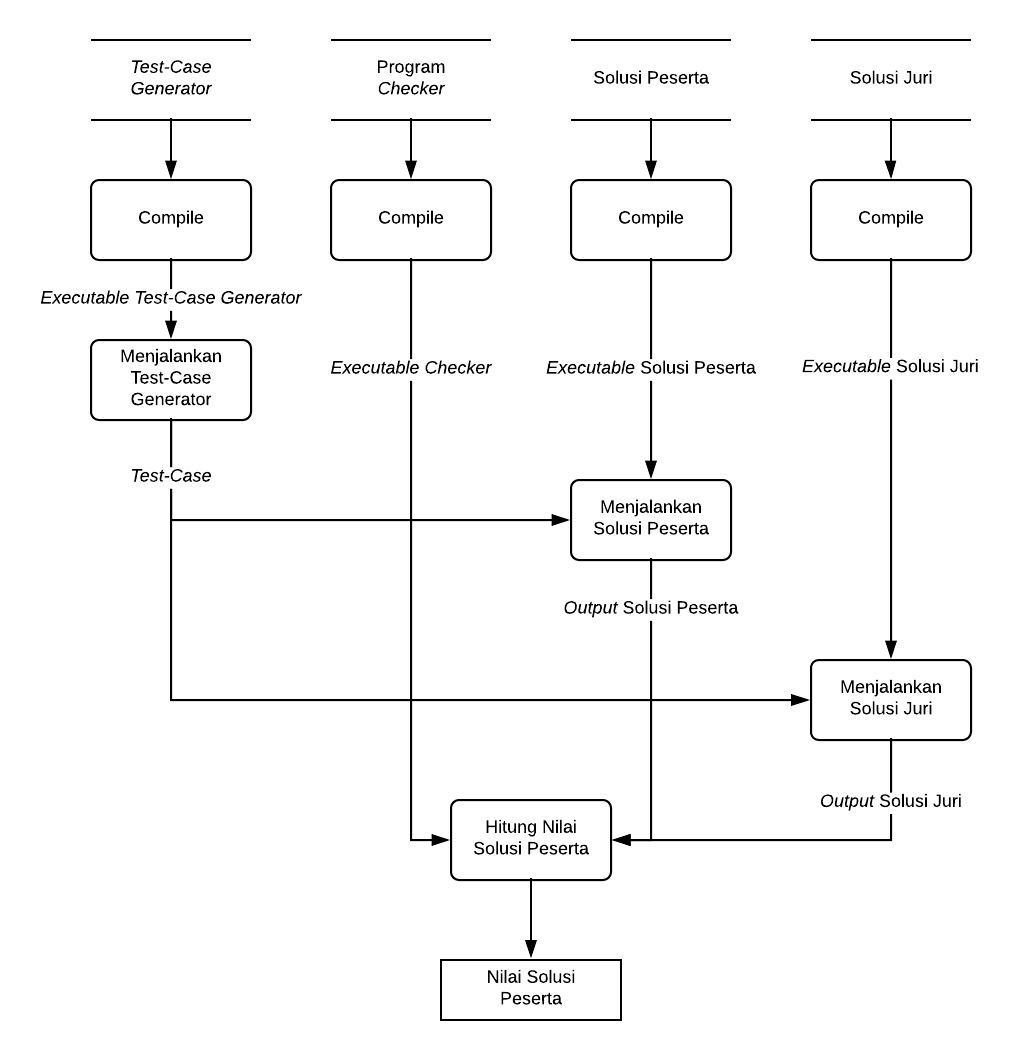
\includegraphics[width=0.85\textwidth]{images/grading-dfd}
    \caption{Diagram Aliran Data Pada Proses Penilaian Solusi Peserta}
    \label{fig:grading-dfd}
\end{figure}

\par Dengan menggunakan TCP dan TLS, kebocoran informasi yang dikirimkan melalui jaringan dapat dihindari sehingga tidak ada pihak ketiga yang dapat mengetahui isi dari informasi tersebut. Akan tetapi, karena informasi ini diterima oleh komputer peserta, peserta dapat dengan mudah mengetahui isi dari informasi tersebut. Oleh karena itu, diperlukan satu lapisan enkripsi lagi pada aplikasi yang berjalan pada komputer peserta. Untuk mencegah peserta mengetahui kunci yang digunakan oleh aplikasi pada komputernya, algoritma pertukaran kunci seperti \textit{Diffie-Hellman} dapat digunakan.

\begin{figure}
    \centering
    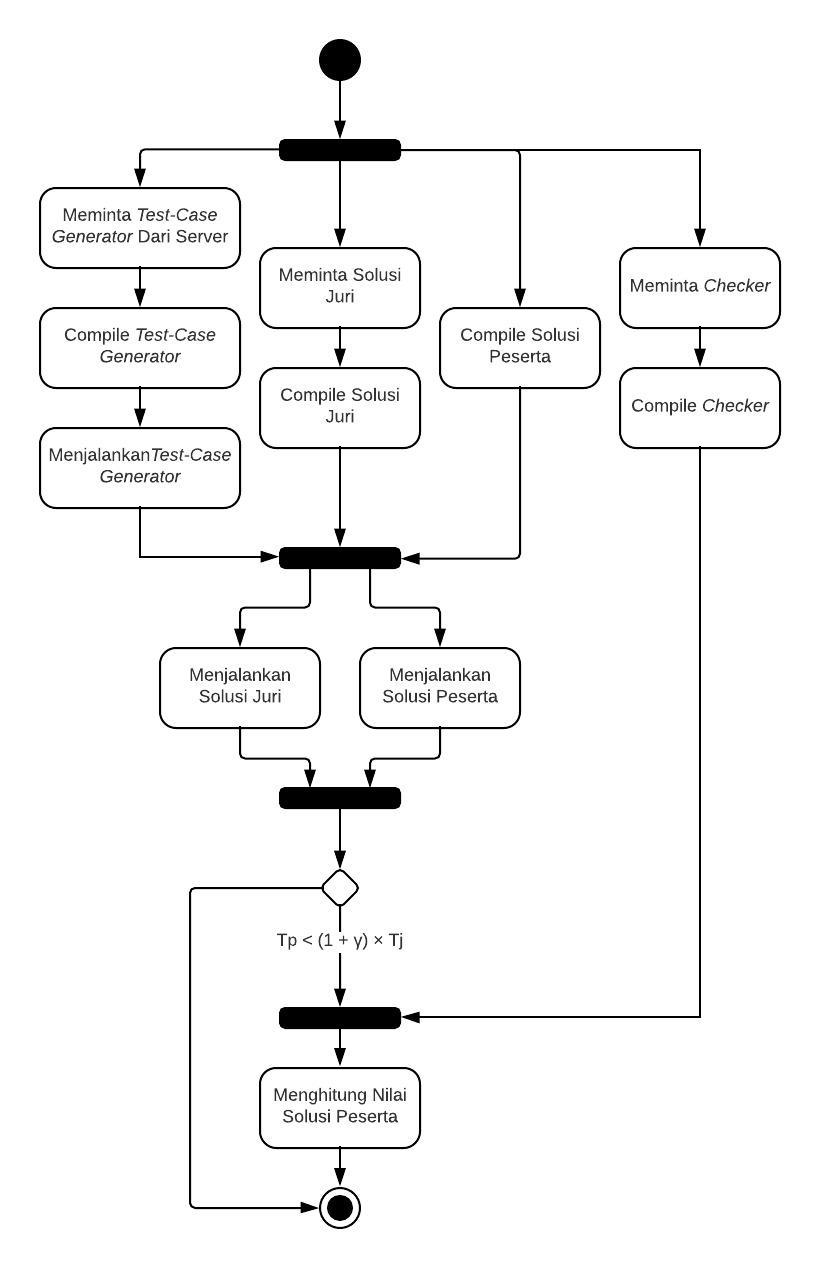
\includegraphics[width=0.65\textwidth]{images/total-grader-activity}
    \caption{Alur Proses Penilaian Jawaban Peserta}
    \label{fig:total-grader-activity}
\end{figure}

\par \textit{Test-case} umumnya merupakan file \textit{text} yang cukup besar. Pengiriman file ini dapat menghabiskan banyak \textit{bandwidth}. Meskipun begitu, \textit{test-case} biasanya dibuat dengan cara dibangkitkan oleh sebuah program yang dibuat oleh juri. \textit{Test-case} yang sama dapat dibangkitkan berulang-kali dengan menjalankan program tersebut. Untuk mengurangi kebutuhan \textit{bandwidth}, \textit{test-case} tidak perlu dikirim, melainkan program pembangkit \textit{test-case} saja yang dikirim. \textit{Test-case} yang akan digunakan untuk melakukan penilaian solusi peserta dibangkitkan dengan program pembangkit \textit{test-case} ini seperti pada gambar \ref{fig:grading-dfd}. Diagram pada gambar \ref{fig:total-grader-activity} menggambarkan alur proses penilaian jawaban peserta secara lengkap.

\par Pada Tugas Akhir ini, \textit{test-case} dipertukarkan dengan mengirimkan program pembangkit \textit{test-case} secara aman. Keamanan diperoleh dengan menggunakan dua kali enkripsi yaitu pada lapisan \textit{transport} dan aplikasi. Terdapat beberapa protokol yang dapat digunakan dalam melakukan pengiriman informasi ini. Protokol yang dipilih pada Tugas Akhir ini adalah protokol yang berbasis RPC yaitu \textit{GRPC}. Protokol ini dipilih karena aman dan mudah untuk digunakan.

\section{Sistem Manajemen Kompetisi}

\par Sistem manajemen kompetisi memberikan layanan kepada peserta kompetisi dan juri untuk berinteraksi. \textit{Online judge} yang populer pada saat ini memberikan sistem manajemen kompetisi berbasis web. Sistem manajemen kompetisi ini dibutuhkan oleh peserta dan juri untuk melakukan aksi-aksi terkait kompetisi yang sedang berlangsung. Kebutuhan dari sistem manajemen kompetisi digambarkan oleh diagram \textit{use case} pada gambar \ref{fig:oj-use-case}.

\begin{figure}[ht!]
    \centering
    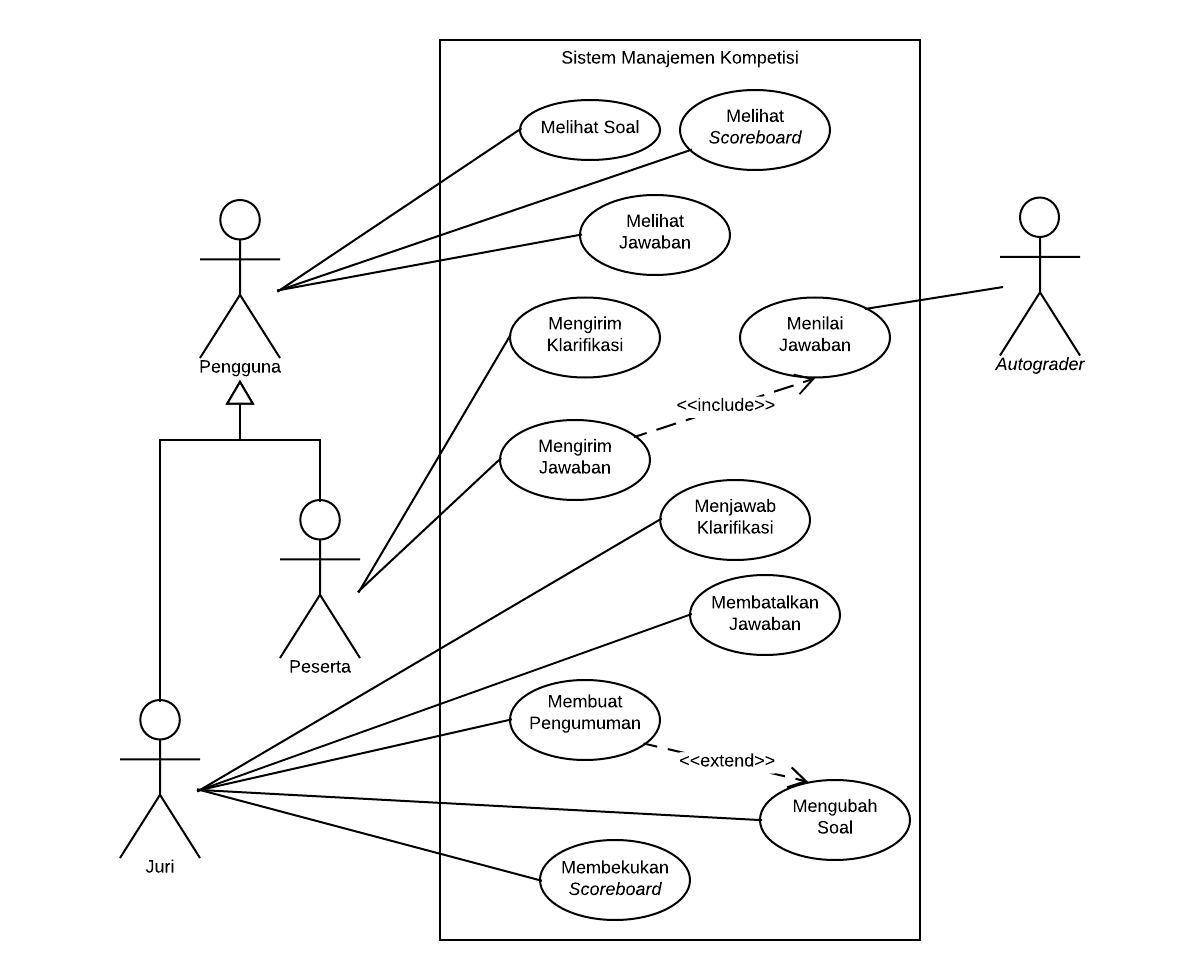
\includegraphics[width=0.85\textwidth]{images/oj-use-case}
    \caption{Diagram \textit{Use Case} Dari Sistem Manajemen Kompetisi}
    \label{fig:oj-use-case}
\end{figure}

\begin{enumerate}
    \item Peserta dan juri dapat melihat soal.
    \item Peserta dapat mengirim jawaban.
    \item Sistem dapat menilai jawaban peserta.
    \item Peserta dapat mengirim klarifikasi soal.
    \item Juri dapat membuat pengumuman terkait kompetisi.
    \item Juri dapat menjawab klarifikasi peserta.
    \item Juri dapat mengubah soal.
    \item Peserta dan juri dapat melihat \textit{scoreboard}.
    \item Juri dapat membekukan \textit{scoreboard}.
    \item Peserta dapat melihat jawaban yang dikirim olehnya.
    \item Juri dapat melihat jawaban yang dikirim seluruh peserta.
    \item Juri dapat mengatur jawaban peserta untuk tidak dinilai.
\end{enumerate}

\begin{figure}[ht!]
    \centering
    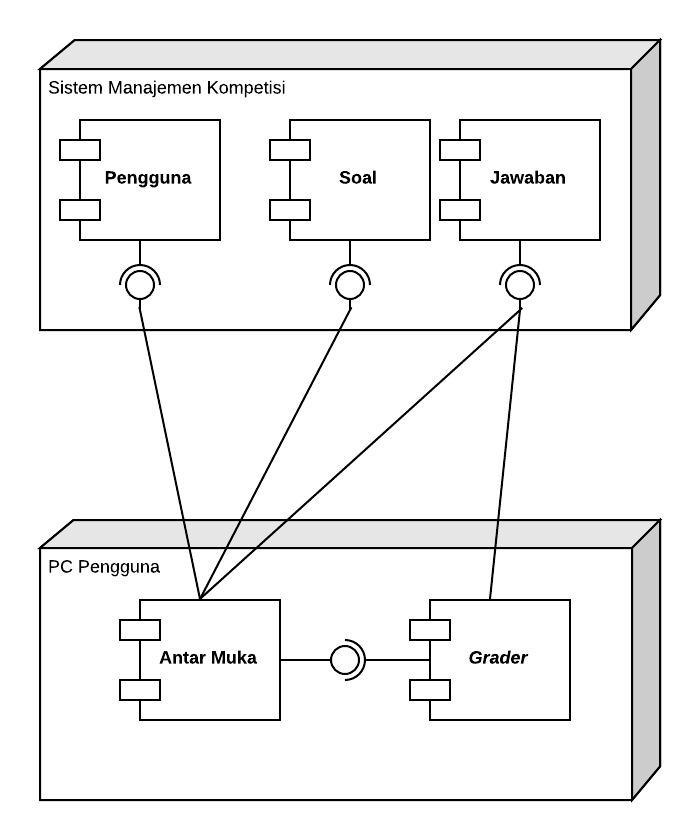
\includegraphics[width=0.85\textwidth]{images/oj-components}
    \caption{Diagram Komponen Sistem Manajemen Kompetisi}
    \label{fig:oj-components}
\end{figure}

\par Masalah yang ingin diselesaikan dalam Tugas Akhir ini tidak terletak pada sistem manajemen kompetisi, melainkan pada sistem \textit{autograder}. Oleh karena itu, sistem manajemen kompetisi yang akan digunakan akan mengikuti sistem manajemen kompetisi yang saat ini banyak digunakan. Sistem manajemen kompetisi ini dapat dibagi menjadi beberapa komponen utama yaitu: pengguna, soal, jawaban, klarifikasi, scoreboard, dan grader. Diagram komponen pada gambar \ref{fig:oj-components} menggambarkan komponen yang akan digunakan dalam sistem manajemen kompetisi beserta keterhubungannya.

\subsection{Komponen Pengguna}

\par Kompetisi \textit{competitive programming} ada yang bersifat tertutup dimana hanya peserta tertentu yang dapat mengikutinya dan terbuka dimana setiap orang dapat mengikutinya. Sistem \textit{online judge} yang populer saat ini umumnya dapat menangani kedua jenis kompetisi tersebut. Untuk memasuki kompetisi, peserta akan terlebih dahulu membuat akun di sistem \textit{online judge} tersebut. Peserta kemudian dapat memasuki kompetisi dengan cara melakukan \textit{login} pada sistem tersebut. Untuk melakukan pendaftaran peserta baru dan \textit{login}, sistem \textit{online judge} perlu memiliki komponen manajemen pengguna yang bertugas melakukan otentikasi dan otorisasi pengguna. Beberapa \textit{online judge} memiliki komponen manajemen pengguna yang memanfaatkan layanan otentikasi dan otorisasi dari pihak ketiga seperti Google, Facebook, Github, dan Auth0. Terdapat juga sistem \textit{online judge} yang melakukan otentikasi dan otorisasi tanpa menggunakan pihak ketiga, misalnya DomJudge dan Mooshak.

\par Komponen pengguna akan dibuat pada sistem manajemen kompetisi untuk melakukan otentikasi dan otorisasi pengguna. Untuk menyederhanakan persoalan, pada Tugas Akhir ini komponen pengguna yang bertugas melakukan otentikasi dan otorisasi pengguna tidak akan menggunakan layanan pihak ketiga. Beberapa \textit{software development framework} seperti Django, Express, dan Laravel memiliki kemampuan untuk menangani masalah ini dengan mudah. Informasi pengguna akan disimpan pada sistem basis data yang sudah tersedia. Otentikasi pengguna akan dilakukan dengan sederhana, yaitu menggunakan \textit{username} dan \textit{password}.

\par Otorisasi pengguna juga akan dilakukan secara sederhana dengan sistem \textit{Role-based access control}. Setiap pengguna akan diberikan \textit{role} tertentu. Aksi-aksi yang dapat dilakukan oleh pengguna ditentukan oleh \textit{role} yang dimilikinya. Role yang akan digunakan dalam sistem manajemen kompetisi ini adalah "peserta" dan "juri". Setiap pengguna yang berhasil \textit{login} kedalam sistem akan diberikan \textit{token} unik. Token unik ini digunakan untuk menentukan \textit{role} dari pengguna yang melakukan aksi pada sistem. \textit{Token} yang akan digunakan dalam Tugas Akhir ini adalah \textit{JWT (JSON Web Token)} karena mudah untuk digunakan dan aman.

\subsection{Komponen Soal}

\par Pada kompetisi \textit{competitive programming}, deskripsi soal dapat diakses melalui sistem \textit{online judge} yang biasanya berupa halaman web. Dalam beberapa kompetisi, peserta kompetisi akan mendapatkan \textit{hard-copy} dari soal. Komponen soal dibutuhkan oleh sistem manajemen kompetisi untuk mengelola soal yang ada pada kompetisi. Komponen ini memberikan layanan kepada pengguna untuk melihat soal. Terkadang terdapat kesalahan pada soal ketika kompetisi berlangsung sehingga komponen ini perlu memberikan layanan kepada juri untuk mengganti soal.

\par Soal pada kompetisi \textit{competitive programming} memiliki deskripsi yang merupakan penjelasan terhadap masalah yang harus diselesaikan peserta. Pada deskripsi soal terdapat penjelasan mengenai permasalahan yang dimaksud, format masukan, format keluaran, contoh masukan, dan contoh keluaran. \textit{Online judge} yang populer saat ini memberikan deskripsi soal kepada peserta dengan format \textit{pdf} atau menampilkannya dalam halaman web. Komponen soal perlu menyimpan deskripsi soal untuk dapat memberikannya kepada pengguna. Deskripsi soal dapat disimpan pada \textit{filesystem} dalam bentuk pdf atau disimpan dalam database dalam bentuk HTML. Untuk memudahkan implementasi pada Tugas Akhir ini, deskripsi soal akan disimpan dalam basis data.

\par Setiap soal perlu memiliki program \textit{test-case generator}, \textit{solution}, dan \textit{checker}. Ketiga buah program ini dibuat oleh juri untuk melakukan penilaian jawaban peserta. \textit{Test-case generator} adalah program yang dibuat oleh juri untuk membangkitkan \textit{test-case} seperti yang sudah dijelaskan pada bagian \ref{subsec:sending-test-case-to-worker}. \textit{Solution} adalah program yang merupakan solusi valid dari soal. Program solusi ini dibuat oleh juri untuk dibandingkan dengan jawaban peserta seperti yang sudah dijelaskan pada bagian \ref{subsec:time-memory-measure-compare-with-jury}. Program \textit{checker} akan digunakan oleh \textit{worker} untuk menentukan kebenaran jawaban peserta. Terkadang terdapat lebih dari satu jawab yang benar pada sebuah soal. Oleh karena itu, program \textit{checker} ini dibutuhkan untuk menilai jawaban peserta. 

\par Program \textit{test-case generator}, \textit{solution}, dan \textit{checker} dapat disimpan dalam \textit{filesystem} atau sistem basis data. Untuk memudahkan implementasi pada Tugas Akhir ini, ketiga program ini akan disimpan dalam bentuk \textit{source code} pada sistem basis data.

\subsection{Komponen Jawaban}

\par Sistem manajemen kompetisi perlu menyediakan layanan kepada peserta untuk mengirimkan jawaban. Jawaban yang dikirimkan peserta berupa program dalam bentuk \textit{source code} dalam bahasa pemrograman yang diizinkan oleh juri. Selain itu, sistem manajemen kompetisi juga harus memberikan layanan kepada peserta untuk dapat melihat kembali jawabannya. Juri juga perlu mengawasi jawaban dari peserta untuk menghindari adanya kecurangan.  Oleh karena itu, sistem manajemen kompetisi juga harus dapat memberikan layanan kepada juri untuk melihat seluruh jawaban yang pernah dikirimkan oleh peserta. Untuk memudahkan implementasi, pada Tugas Akhir ini jawaban peserta akan disimpan dalam bentuk \textit{source code} pada sistem basis data.

\subsection{Komponen Klarifikasi}

\par Dalam kompetisi \textit{competitive programming}, terkadang terdapat deskripsi soal yang salah atau kurang jelas. Oleh karena itu, perlu adanya sistem yang dapat memberikan layanan kepada juri dan peserta untuk saling berinteraksi. Sistem interaksi ini dapat memberikan layanan kepada juri untuk memberikan pengumuman terkait keberjalanan kompetisi. Selain itu, sistem interaksi ini dapat memberikan layanan kepada peserta untuk mengajukan pertanyaan terkait soal ataupun keberjalanan kompetisi kepada juri. Juri dapat menjawab pertanyaan peserta melalui sistem interaksi ini.

\begin{figure}[ht!]
    \centering
    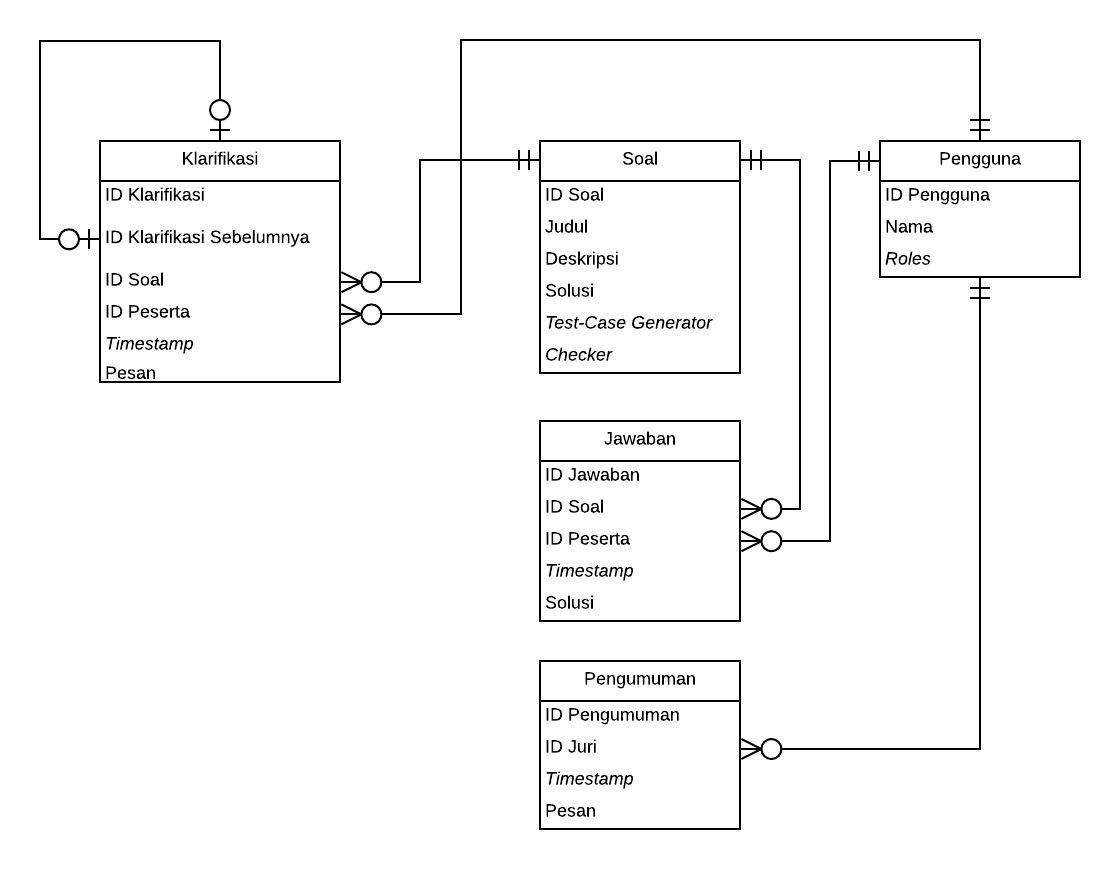
\includegraphics[width=0.9\textwidth]{images/oj-erd}
    \caption{Skema Basis Data Sistem Manajemen Kompetisi}
    \label{fig:oj-erd}
\end{figure}

\par Interaksi yang terjadi antara peserta dengan juri dilakukan dengan pengiriman pesan teks singkat. Pada Tugas Akhir ini, interaksi antara peserta dan juri akan disimpan dalam sistem basis data. Gambar \ref{fig:oj-erd} menggambarkan skema basis data yang akan digunakan pada sistem manajemen kompetisi yang akan dikembangkan.

\subsection{Komponen \textit{Scoreboard}}

\par \textit{Scoreboard} merupakan halaman yang berisi peringkat peserta pada kompetisi yang sedang berlangsung. Halaman ini memberikan informasi kepada peserta, juri, maupun orang di luar kompetisi mengenai jumlah soal yang berhasil dikerjakan setiap peserta, jumlah jawaban yang dikirimkan tiap peserta, maupun peringkat peserta. Peringkat peserta dihitung dengan cara tertentu, misalnya dengan jumlah soal yang berhasil dijawab dengan benar.

\par Perhitungan peringkat pada sistem manajemen kompetisi dapat dikategorikan sebagai pekerjaan yang berat. Hal ini dikarenakan, peringkat harus selalu diperbarui ketika terdapat peserta yang mengirimkan jawaban. \textit{Online judge} yang populer saat ini biasanya melakukan perhitungan peringkat secara periodik. Hal ini menyebabkan informasi peringkat tidak diperbarui secara \textit{realtime}. Pada Tugas Akhir ini, perhitungan peringkat akan diserahkan kepada komputer peserta sendiri sehingga tidak membebani \textit{server} dengan perhitungan yang berat.
